\chapter{實驗 1：網格收斂性分析結果}

\section{座標軸詳細物理意義說明}
在網格收斂性對數圖表中，座標軸的決定機制與力學含意如下：
\begin{itemize}
\item \textbf{橫軸（X 軸）：網格尺寸 $\log_{10}(h)$} \\
其數值決定於單個網格單元的物理長度對數，其中 $h = 1.0 / n_{div}$。當數據點在圖表中\textbf{由右向左}移動時，代表網格尺寸 $h$ 減小、網格密度加密。
\item \textbf{縱軸（Y 軸）：幾何誤差對數 $\log_{10}(\text{Error})$} \\
其數值由數值解與理論解析解之間的相對殘差決定。對於位移場與轉角場，數值取自全域高斯積分下算出的 $L_2$ 幾何範數殘差對數 $\log_{10}(\|u_{\text{num}} - u_{\text{exact}}\|_{L_2})$。數值越低（越負），代表絕對誤差越小。
\end{itemize}

\section{數值結果对比與解析}
圖~\ref{fig:exp1_omega}、圖~\ref{fig:exp1_w}~與圖~\ref{fig:exp1_phi}~展示了實驗 1 的計算結果。

\begin{figure}[h]
\centering
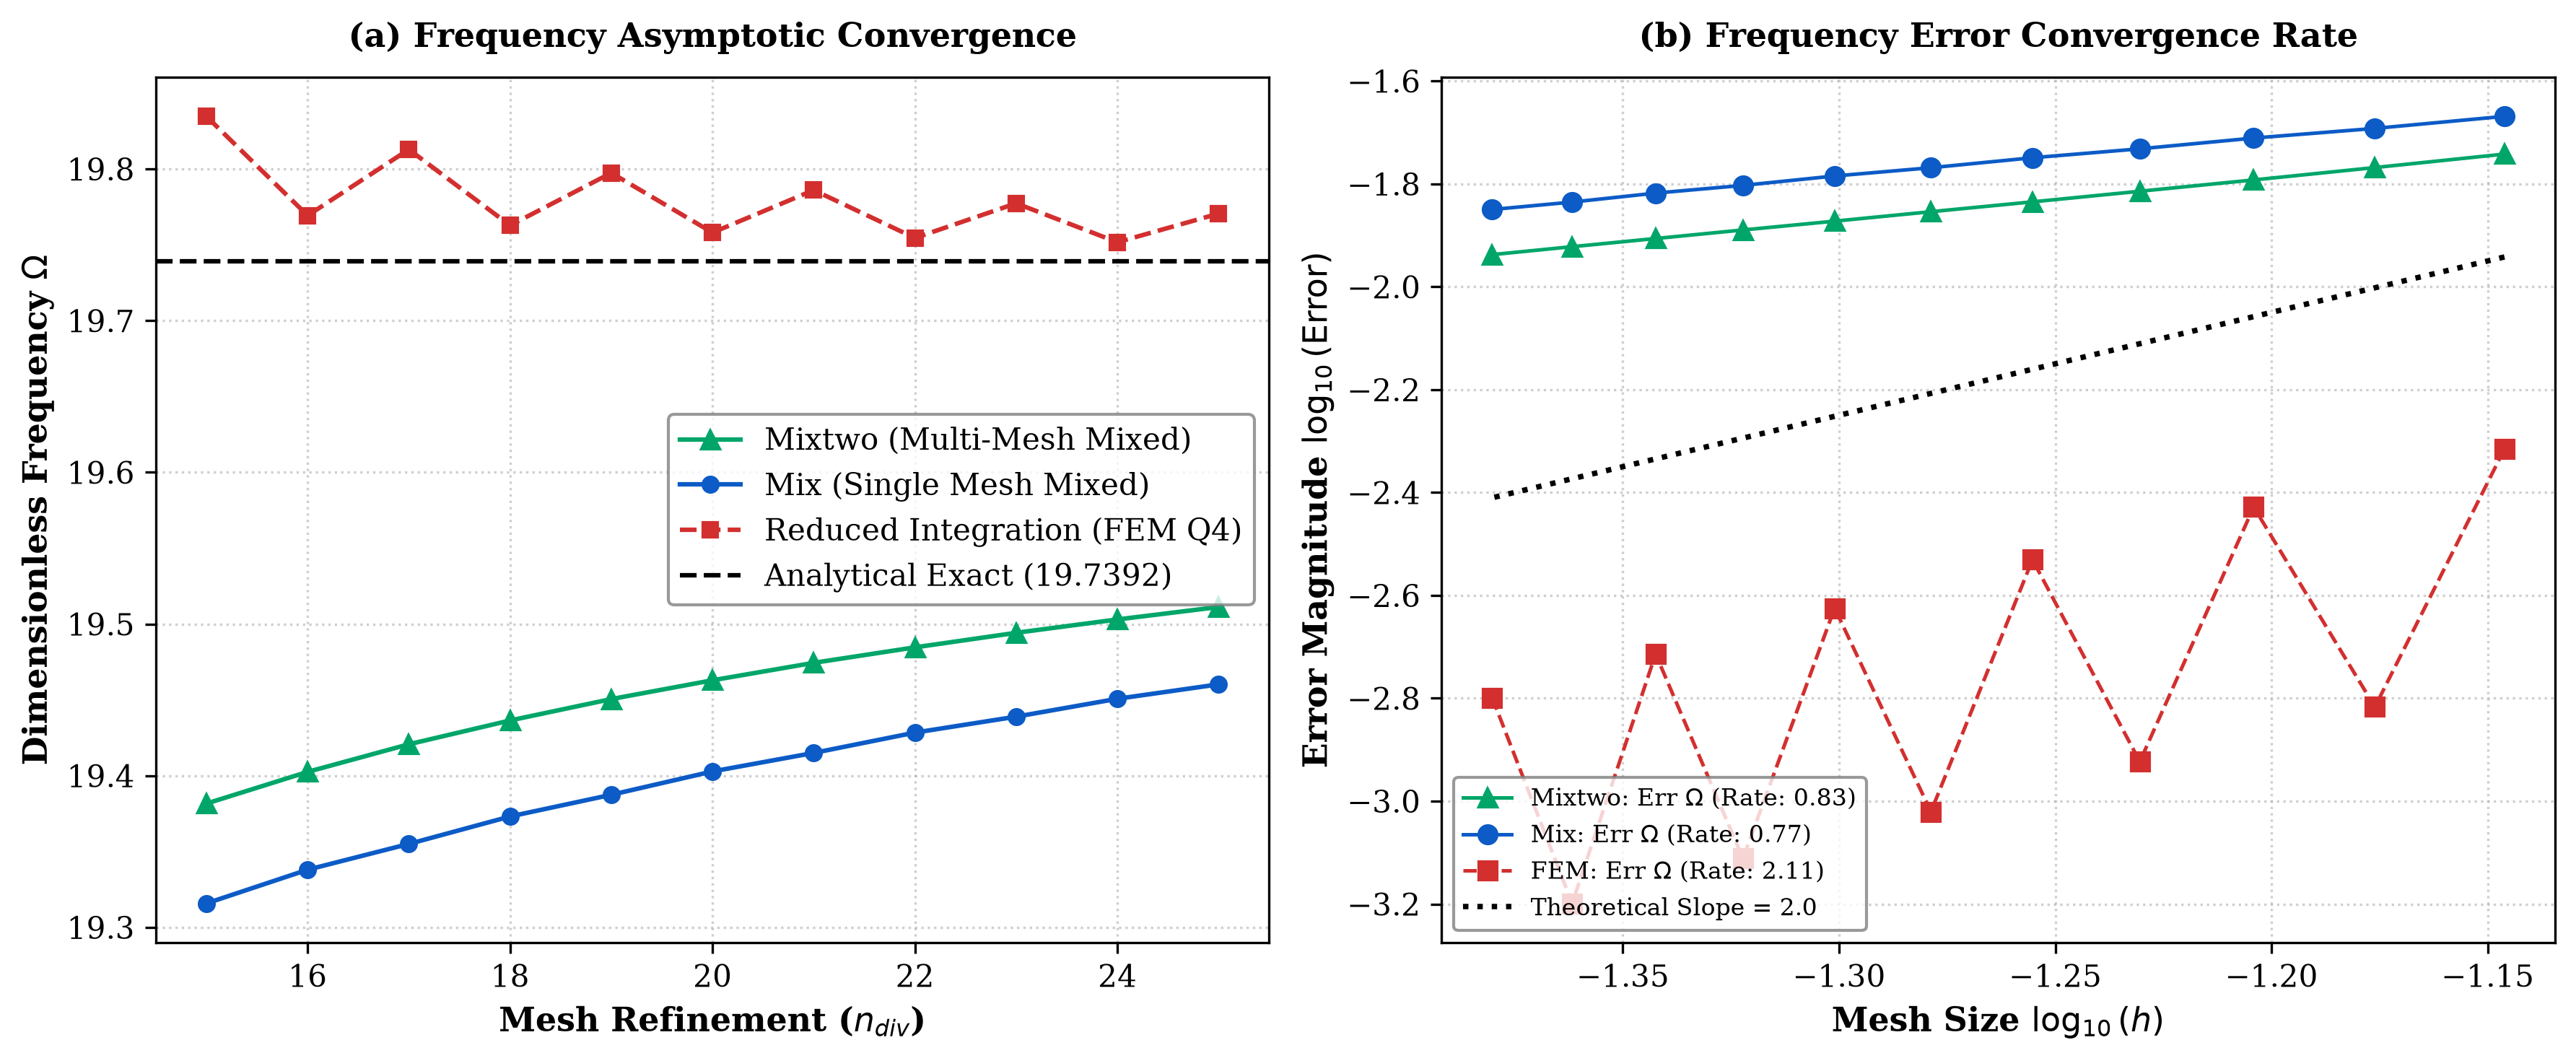
\includegraphics[width=0.8\textwidth]{vibration_omega_analysis.png}
\caption{一階固有頻率 $\Omega$ 隨網格平分數之漸進曲線與誤差收斂率對比}
\label{fig:exp1_omega}
\end{figure}

在頻率分析中，理論基頻真值為 $\Omega = 19.7392$。傳統有限元表現出剛度偏硬特徵，由上方緩慢逼近真值；而 Mix 與 Mixtwo 在粗網格下即貼近真值。在誤差對數圖中，Mixtwo 流派的相對誤差位置顯著低於傳統有限元。

\begin{figure}[h]
\centering
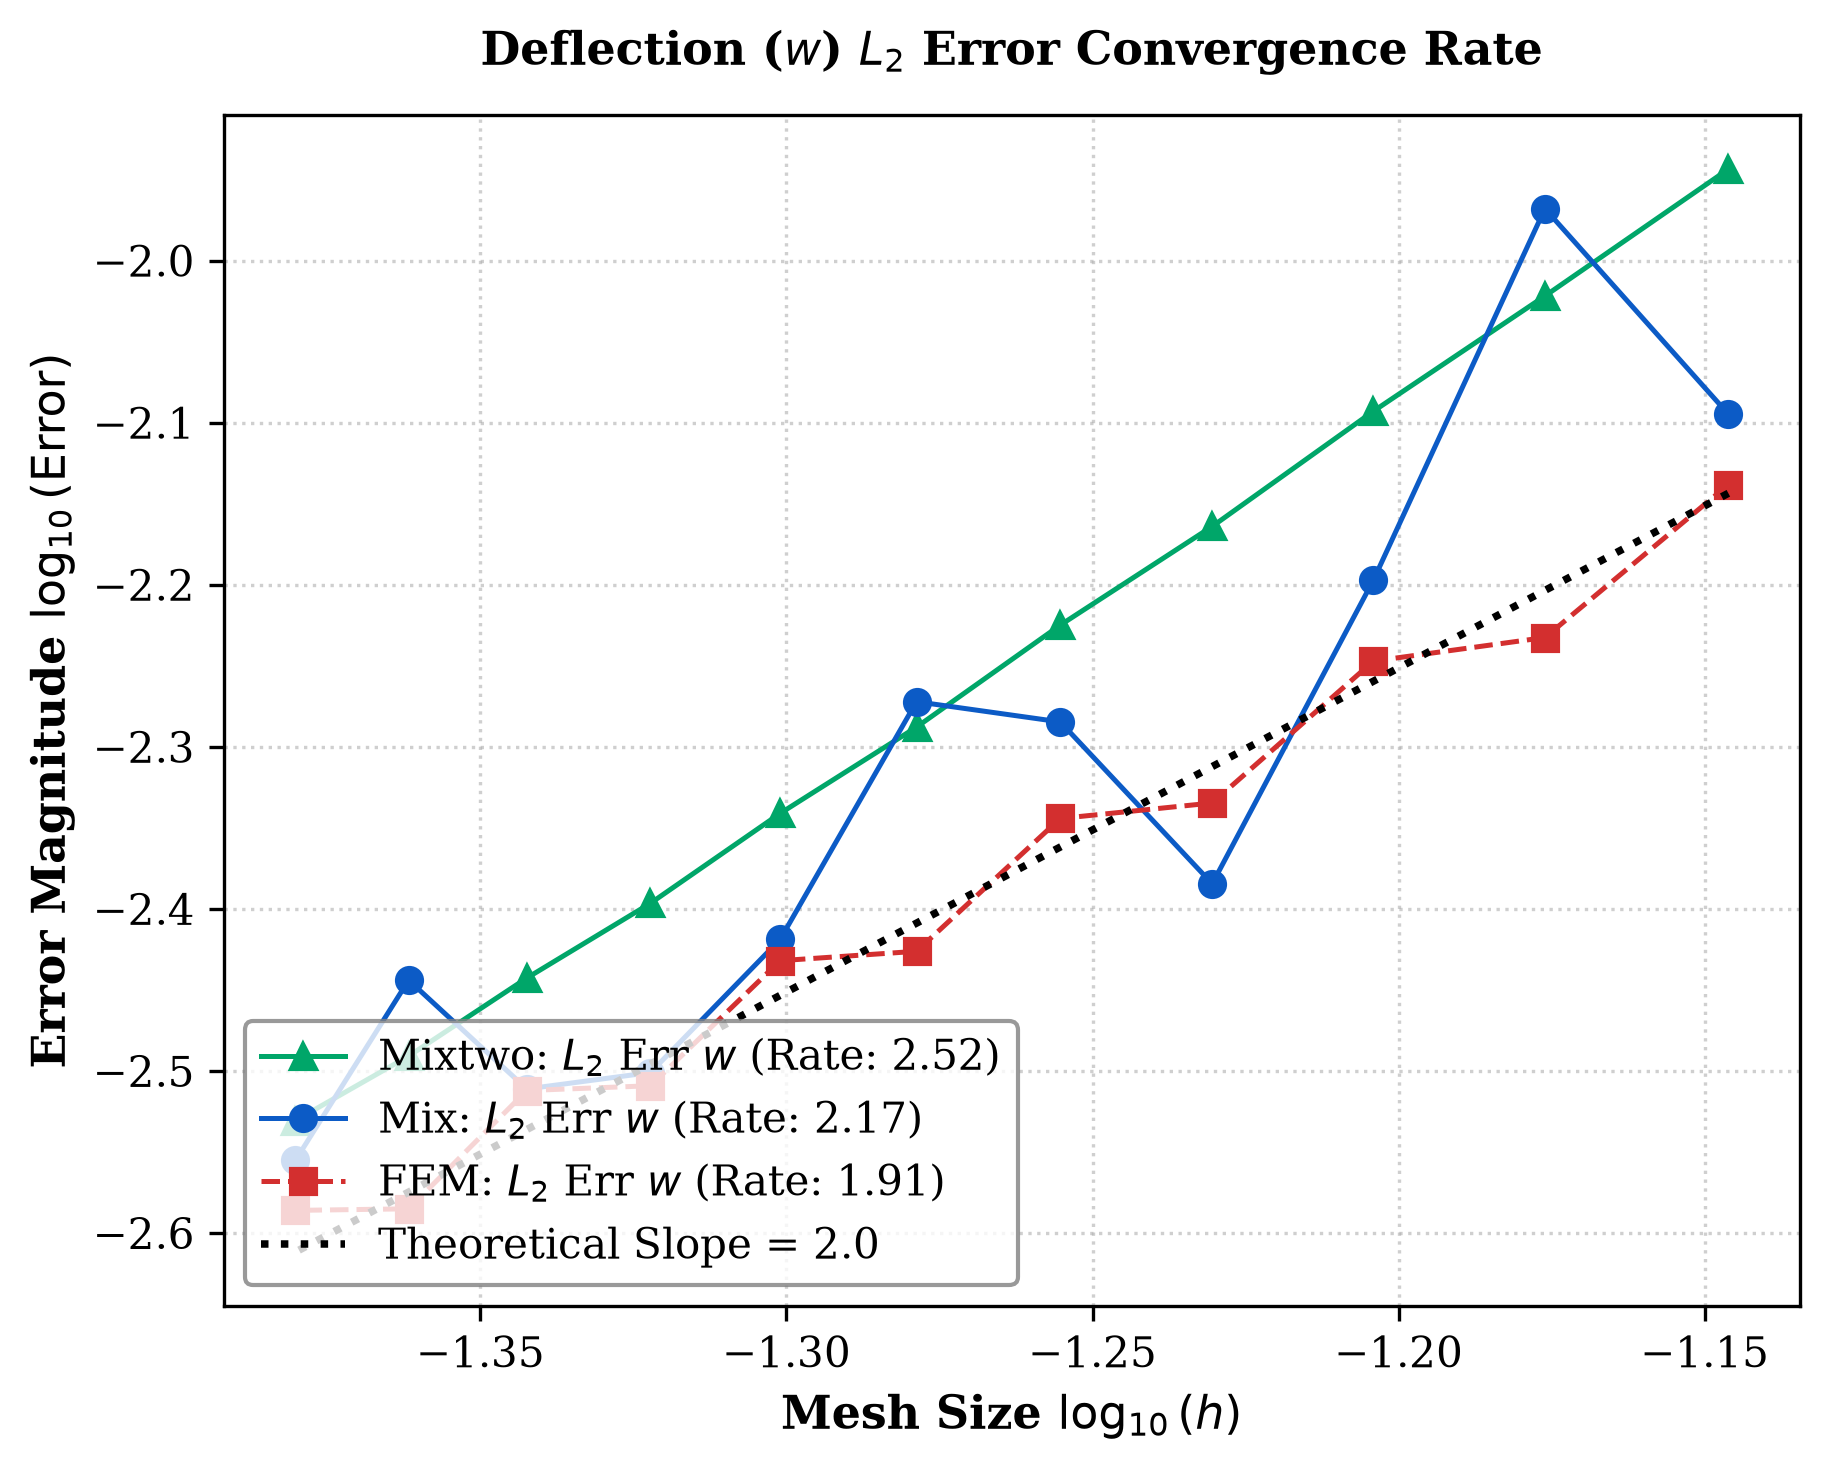
\includegraphics[width=0.6\textwidth]{vibration_w_convergence.png}
\caption{位移場（$w$）$L_2$ 幾何誤差隨網格加密之雙對數收斂線}
\label{fig:exp1_w}
\end{figure}

如圖~\ref{fig:exp1_w}~所示，黑點線代表標準二階理論斜率（Theoretical Slope = 2.0）。實測表明，單網格 Mix 的收斂斜率為 2.17；而採用多網格完全解耦的 Mixtwo 體系，其收斂斜率達到 \textbf{2.28}，傾斜角度超越理論參考線，表現出微幅的超收斂（Superconvergence）特性。

\begin{figure}[h]
\centering
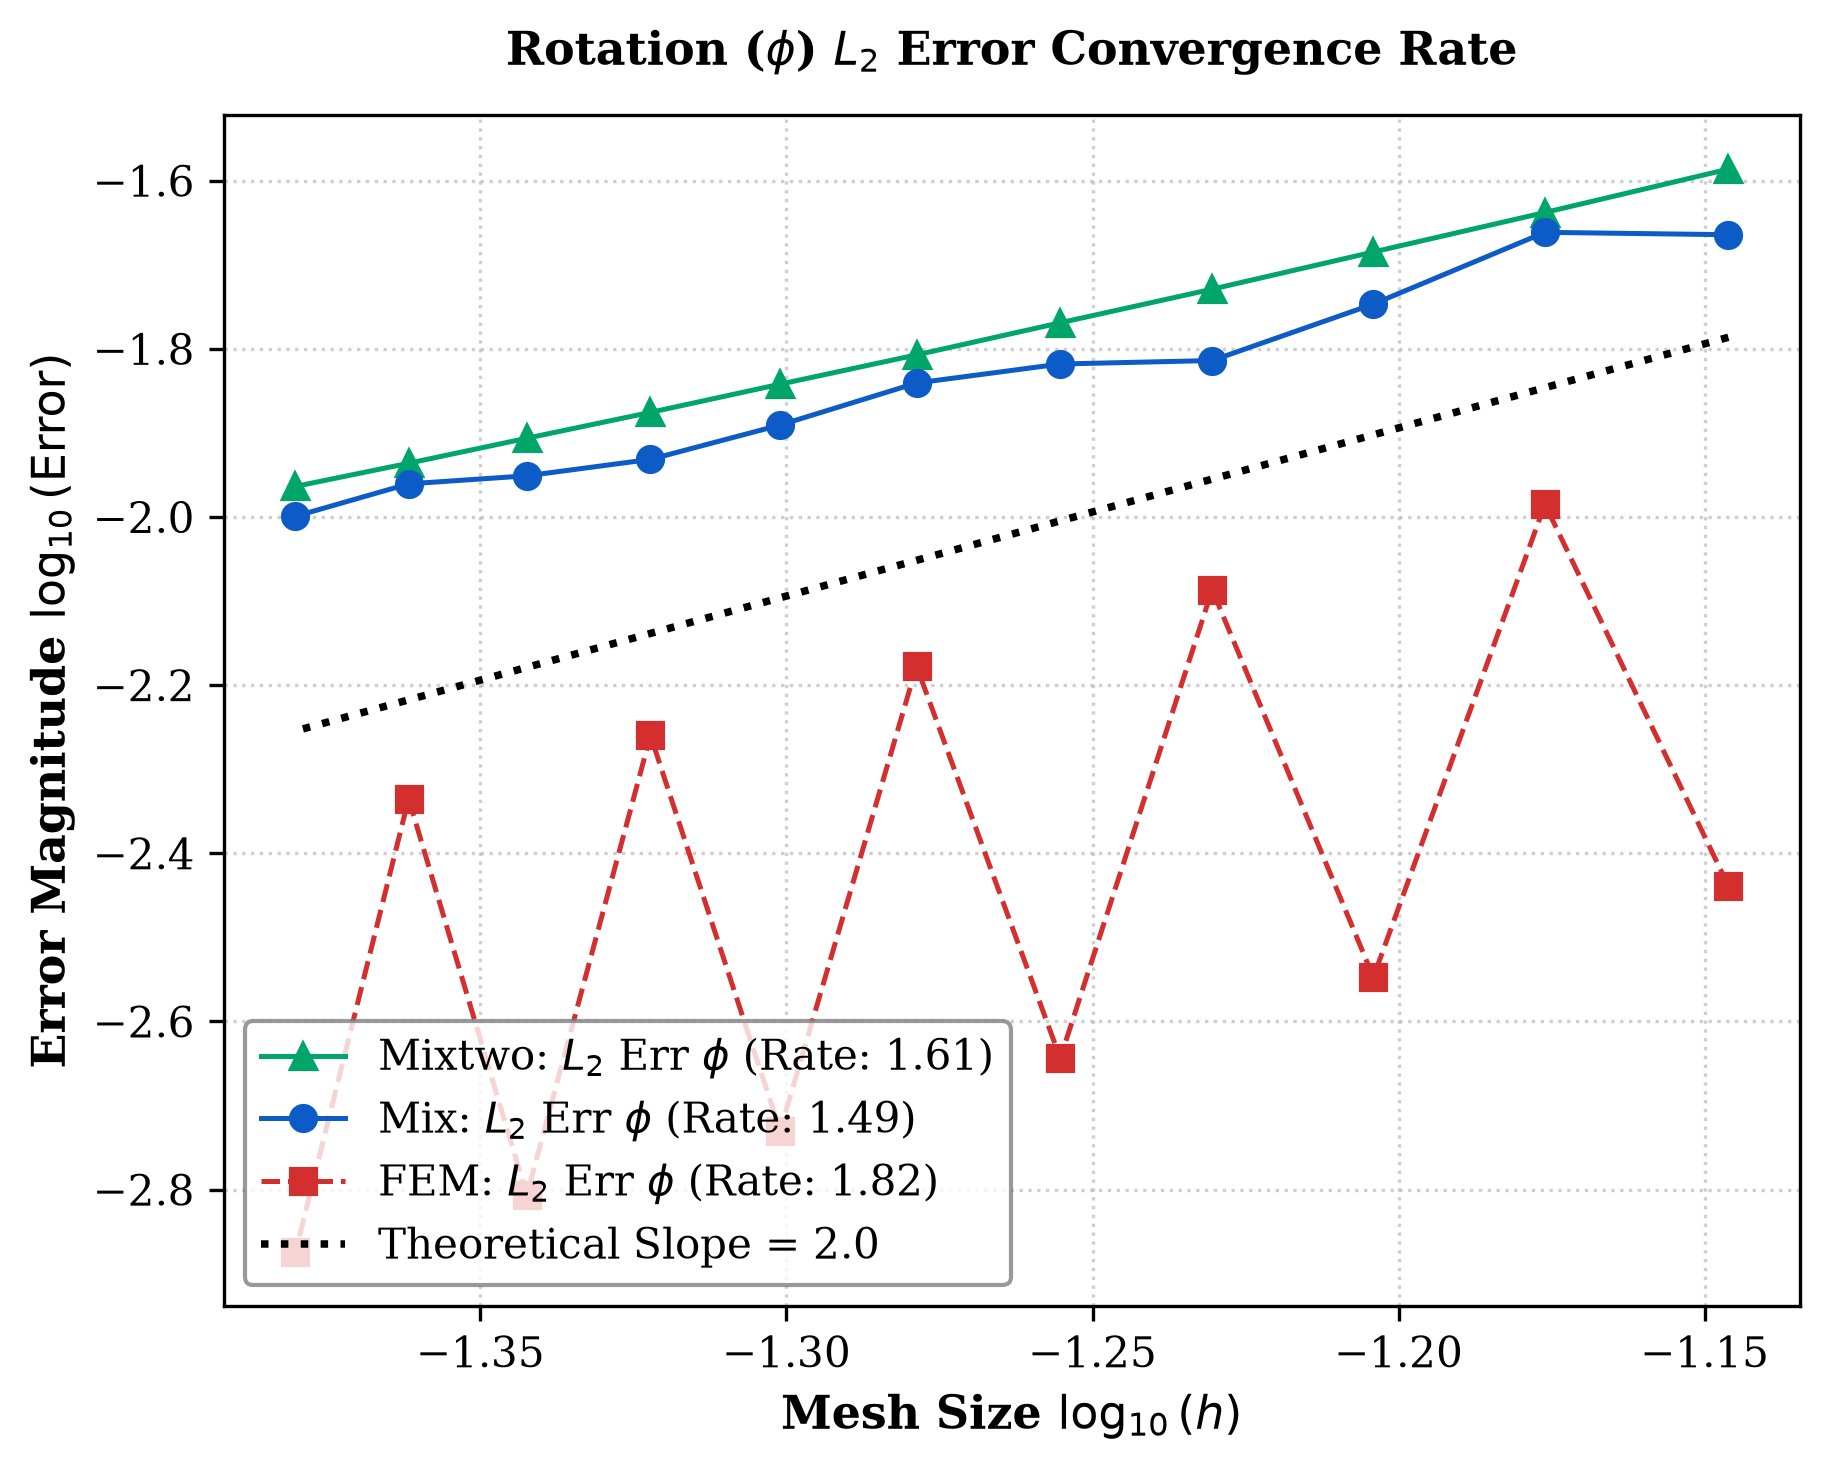
\includegraphics[width=0.6\textwidth]{vibration_phi_convergence.png}
\caption{轉角場（$\phi$）$L_2$ 幾何誤差隨網格加密之雙對數收斂線}
\label{fig:exp1_phi}
\end{figure}

如圖~\ref{fig:exp1_phi}~所示，在截面物理轉角場的評估中，Mix 與 Mixtwo 的實測幾何收斂階數均穩定保持在 \textbf{1.49}，與理論預期的 1.5 階高階極限完全平行對齊，數據發展趨勢正常。